\providecommand\ExamFontPath{../../../字体/}
\documentclass[fontset=exam]{exam-zh}
\usepackage{longtable,booktabs,array,calc,multirow,fvextra}
\usepackage[normalem]{ulem}
\providecommand{\hl}[1]{#1}
\providecommand{\ul}[1]{\uline{#1}}
\DefineVerbatimEnvironment{verbatim}{Verbatim}{breaklines=true,fontsize=\small}
\providecommand{\tightlist}{\setlength{\itemsep}{0pt}\setlength{\parskip}{0pt}}
\newcommand{\pandocbounded}[1]{#1}
\setlength{\emergencystretch}{3em}
\setlength{\tabcolsep}{2pt}
\examsetup{page/size=a4paper}
\title{厦门大学期中考试 A 卷}
\subject[9em]{大学物理 B（下）}
\begin{document}
\maketitle
\fancyfoot[C]{第 \thepage 页（共 \pageref*{LastPage} 页）}
\noindent\makebox[\linewidth][c]{考试时间：2024 年 11 月}\par
\pdfbookmark[1]{一、选择题：本题共10小题，每小题2分，共20分。请把正确答案填写在答题纸的正确位置。每小题给出的四个选项中只有一个选项}{section4}

\par\medskip{\heiti

一、选择题：本题共 10 小题，每小题 2 分，共 20 分。请把正确答案填写在答题纸的正确位置。每小题给出的四个选项中只有一个选项正确。错选、多选或未选的得 0 分。

\par}\smallskip

1. 在用电场线形象描述静电场的表述中，电场线方向就是（ ）

（A）电势能减小的方向 （B）电势减小最快的方向

（C）正电荷在电场中的运动方向 （D）负电荷在电场中的运动力向

2. 真空中有两个平行的无限大均匀带电平面，电荷面密度分别为−\emph{σ}和−2\emph{σ} 。如图所示，两平面之间\emph{A}、\emph{B}两点的电势分别为\emph{V\textsubscript{A}}、\emph{V\textsubscript{B}}，则（ ）\par\medskip{\centering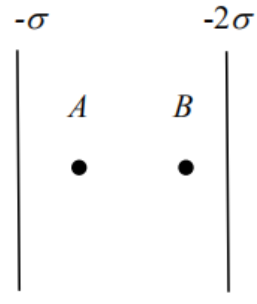
\includegraphics[width=5cm,height=4cm,keepaspectratio]{figures/image1.png}\par}\medskip

（A）\emph{V\textsubscript{A}} \textgreater{} \emph{V\textsubscript{B}} （B）\emph{V\textsubscript{A}} \textless{} \emph{V\textsubscript{B}}

（C）\emph{V\textsubscript{A}} = \emph{V\textsubscript{B}} （D）无法比较二者大小

3. 在半径为\emph{R}的金属球内偏心地挖出一个半径为\emph{r}的球形空腔，腔内距腔心\emph{d}处置一点电荷\emph{q}，金属球带电量为−\emph{q}，则空腔中心的电势为（ ）

\par\medskip{\centering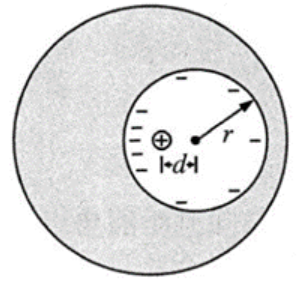
\includegraphics[width=5cm,height=4cm,keepaspectratio]{figures/image2.png}\par}\medskip

（A）0 （B）\(\frac{q}{4\pi\varepsilon_{0}}\left( {\frac{1}{R} - \frac{1}{r}} \right)\)

（C）\(\frac{q}{4\pi\varepsilon_{0}}\left( {\frac{1}{d} - \frac{1}{R}} \right)\) （D）\(\frac{q}{4\pi\varepsilon_{0}}\left( {\frac{1}{d} - \frac{1}{r}} \right)\)

4. 一导体球外充满相对电容率为\emph{ε\textsubscript{r}}的均匀电介质，若测得导体表面之外附近场强为\emph{E}，则导体球面上的自由电荷面密度\emph{σ}为（ ）

（A）\emph{ε}\textsubscript{0}\emph{E} （B）\emph{ε}\textsubscript{0}\emph{ε\textsubscript{r}E} （C）\emph{ε\textsubscript{r}E} （D）(\emph{ε}\textsubscript{0}\emph{ε\textsubscript{r }}- \emph{ε}\textsubscript{0})\emph{E}

5. 把一充电的电容器与一未充电的电容器并联，如果两只电容器的电容完全一样，那么总静电能将（ ）

（A）减小 （B）不变 （C）增大 （D）无法确定

6. 有一半径为\emph{R}、电荷线密度为\emph{λ}的均匀带电圆环, 以角速度\emph{ω}绕其一直径旋转。现将转动圆环置入匀强磁场中, 磁感强度\(\overset{\rightharpoonup}{B}\)与转轴垂直, 则圆环受到的磁力矩大小为（ ）

（A）\(\frac{\pi\lambda\omega BR^{3}}{2}\) （B）\(\frac{\pi\lambda\omega BR^{3}}{\text{4}}\) （C）\(\frac{\pi\lambda\omega BR^{\text{4}}}{2}\) （D）\(\pi\lambda\omega BR^{3}\)

7. 如图所示, 一电子以速度\emph{v}垂直地进入磁感强度为\emph{B}的匀强磁场中, 此电子在磁场中的运动轨道所围面积内的磁通量将（ ）

\par\medskip{\centering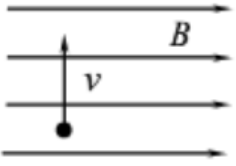
\includegraphics[width=5cm,height=4cm,keepaspectratio]{figures/image11.png}\par}\medskip

（A）正比于\emph{B}, 反比于电子动能 （B）反比于\emph{B}, 正比于电子动能

（C）正比于\emph{B}, 反比于\emph{v} （D）反比于\emph{B}, 反比于\emph{v}

8. 把一根磁矩为\(\overset{\rightharpoonup}{m}\)的条形永磁铁放在磁感应强度为\(\overset{\rightharpoonup}{B}\)的均匀磁场中, 当条形磁铁与\(\overset{\rightharpoonup}{B}\)夹角为\emph{π}/3 时, 它受到的力矩的大小为（ ）

（A）0 （B）\emph{mB} （C）\(\frac{\sqrt{\text{3}}}{\text{2}}\)\emph{mB} （D）\(\frac{\text{1}}{\text{2}}\)\emph{mB}

9. 有两个回路\emph{L}\textsubscript{1}、\emph{L}\textsubscript{2}，其中\emph{L}\textsubscript{1}为图中的小圆环，\emph{L}\textsubscript{2}为由两根直导线与两根弧形导线构成的回路，两回路导线材质相同，大圆环区域内存在磁场，其磁感应强度随时间均匀增加。则以下说法中不正确的是（ ）\par\medskip{\centering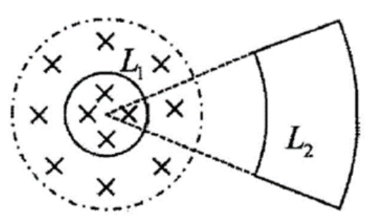
\includegraphics[width=5cm,height=4cm,keepaspectratio]{figures/image15.png}\par}\medskip

（A）回路\emph{L}\textsubscript{1}中有感应电流 （B）回路\emph{L}\textsubscript{2}中有感应电流

（C）回路\emph{L}\textsubscript{1}中电势处处相等 （D）回路\emph{L}\textsubscript{2}中产生了感应电场

10. 横截面为矩形的密绕螺绕环, 总匝数为\emph{N}, 内、外半径分别为\emph{R}\textsubscript{1}和\emph{R}\textsubscript{2}, 厚度为\emph{h}, 则螺绕环的自感\emph{L}=（ ）

（A）\(\frac{\mu_{\text{0}}N^{2}h}{2\pi}ln\frac{R_{2}}{R_{1}}\) （B）\(\frac{\mu_{\text{0}}N^{2}h}{\pi}ln\frac{R_{2}}{R_{1}}\) （C）\(\frac{\mu_{\text{0}}N^{2}h}{2\pi}ln\frac{R_{\text{1}}}{R_{\text{2}}}\) （D）\(\frac{\mu_{\text{0}}N^{2}h}{\pi}ln\frac{R_{\text{1}}}{R_{\text{2}}}\)

\pdfbookmark[1]{二、填空题：本大题共10空，每空2分，共20分。请把正确答案填写在答题纸的正确位置。错填、不填均无分。}{section32}

\par\medskip{\heiti

二、填空题：本大题共 10 空，每空 2 分，共 20 分。请把正确答案填写在答题纸的正确位置。错填、不填均无分。

\par}\smallskip

1. 如图，四个立方体均匀带电，并排放在一起时，在\emph{O}点产生的场强大小为\emph{E}\textsubscript{0}。现去掉其中一个立方体（设其它立方体带电不变），则余下三个立方体在\emph{O}点产生的场强大小为\underline{\hspace{1.5cm}}。\par\medskip{\centering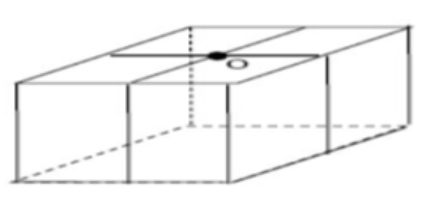
\includegraphics[width=5cm,height=4cm,keepaspectratio]{figures/image21.png}\par}\medskip

2. 四个均匀带电薄球壳的带电量均为\emph{q}，它们的半径分别为\emph{R}、\emph{R}/2、\emph{R}/4、\emph{R}/8，彼此相切于\emph{P}点，球心分别为\emph{O}\textsubscript{1}、\emph{O}\textsubscript{2}、\emph{O}\textsubscript{3}、\emph{O}\textsubscript{4}，则\emph{O}\textsubscript{4}与\emph{O}\textsubscript{1}点的电势差\emph{V}\textsubscript{4}−\emph{V}\textsubscript{1}=\underline{\hspace{1.5cm}}。

\par\medskip{\centering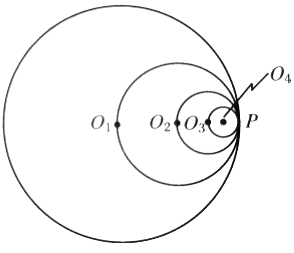
\includegraphics[width=5cm,height=4cm,keepaspectratio]{figures/image24.png}\par}\medskip

3. 如图所示，一金属球半径为\emph{R}，带电−\emph{Q}，距离球心为 3\emph{R}处有一点电荷−\emph{q}。如果选无穷远处为电势零点，则金属球的电势为\underline{\hspace{1.5cm}}。\par\medskip{\centering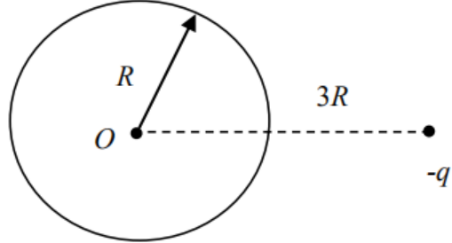
\includegraphics[width=5cm,height=4cm,keepaspectratio]{figures/image25.png}\par}\medskip

4. 一块由无极分子构成的电介质的分子数密度为\emph{n}，在外场的作用下，每个分子感生出来的电偶极矩都相等，都为\(\overset{\rightharpoonup}{p}\)，则介质中电极化强度为\underline{\hspace{1.5cm}}。

5. 真空中有一平行板电容器, 极板面积为\emph{S}, 极板间距为\emph{d}, 极板上分别带有±\emph{Q}的电荷, 则此电容器储存的能量\emph{We}=\underline{\hspace{1.5cm}}。

6. 在同一均匀磁场中, 有两个平面单匝线圈, 其面积\emph{A}\textsubscript{1}=2\emph{A}\textsubscript{2}, 通以电流\emph{I}\textsubscript{1}=2\emph{I}\textsubscript{2}, 则它们所受最大磁力矩之比为\underline{\hspace{1.5cm}}。

7. 如图三根载流导线形成的磁场中，\(\overset{\rightharpoonup}{B}\)沿着图中闭合路径的线积分为 3.77×10\textsuperscript{−6} T\(\cdot\)m，则\emph{I}\textsubscript{3}=\underline{\hspace{1.5cm}}A。\par\medskip{\centering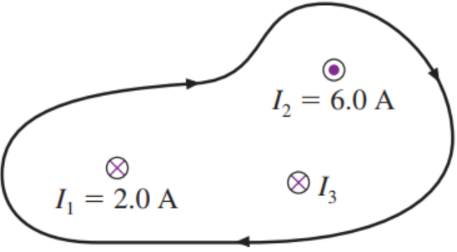
\includegraphics[width=5cm,height=4cm,keepaspectratio]{figures/image27.png}\par}\medskip

8. 北京正负电子对撞机中电子可加速到能量为 2.8×10\textsuperscript{9} eV, 该电子在周长为 240 m 的储存环中作圆周运动, 则维持圆周运动所需要的磁感强度的大小 B=\underline{\hspace{1.5cm}}T。

9. 将一块铜板垂直于磁场方向放在磁场中，磁场的磁感强度随时间减弱，铜板中感应电流产生的磁场与外磁场的方向 。（相同/相反/不确定）

10. 如图，以\emph{a}、\emph{b}为端点的线圈 1 的自感为\emph{L}\textsubscript{1}，以\emph{c}、\emph{d}为端点的线圈 2 的自感为\emph{L}\textsubscript{2}，互感为\emph{M}。若将两线圈 1 和 2 首尾相接（顺接）而串联起来，如图所示，则总自感为\underline{\hspace{1.5cm}}。\par\medskip{\centering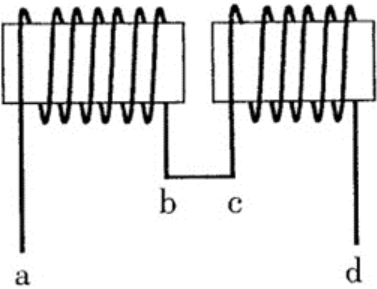
\includegraphics[width=5cm,height=4cm,keepaspectratio]{figures/image29.png}\par}\medskip

\pdfbookmark[1]{三、计算题：本题12分。请在答题纸上按题序作答，并标明题号。}{section45}

\par\medskip{\heiti

三、计算题：本题 12 分。请在答题纸上按题序作答，并标明题号。

\par}\smallskip

内外半径分别为\emph{R}\textsubscript{1}、\emph{R}\textsubscript{2}的带电球层, 电荷体密度为\emph{ρ}=\emph{A}/\emph{r}, 式中\emph{A}是常量, \emph{r}为球壳内任一点到球心的距离。

（1）用电场强度和电势的关系求带电球层外任一点处的电场强度;

（2）将点电荷+\emph{q}从无穷远移到距离球心为\emph{r} (\emph{r} \textgreater{} \emph{R}\textsubscript{2}) 处的\emph{P}点，电场力所做的功是多少?

\pdfbookmark[1]{四、计算题：本题12分。请在答题纸上按题序作答，并标明题号。}{section49}

\par\medskip{\heiti

四、计算题：本题 12 分。请在答题纸上按题序作答，并标明题号。

\par}\smallskip

半径为\emph{R}\textsubscript{1}=1.0 cm 的导体球, 带有电荷\emph{q}=1.0×10\textsuperscript{−10}C, 球外有一个内外半径分别为\emph{R}\textsubscript{2}=3.0 cm

和\emph{R}\textsubscript{3}=4.0 cm 的同心导体球壳, 壳上带有电荷\emph{Q}=1.1×10\textsuperscript{−9}C, 试计算:

（1）两导体的电势\emph{U}\textsubscript{1}和\emph{U}\textsubscript{2}；

（2）用导线把球和球壳接在一起后, \emph{U}\textsubscript{1}和\emph{U}\textsubscript{2}分别是多少?

（3）若外球接地, \emph{U}\textsubscript{1}和\emph{U}\textsubscript{2}为多少?

（4）若内球接地, \emph{U}\textsubscript{1}和\emph{U}\textsubscript{2}为多少? (取无穷远处为电势零点)

\pdfbookmark[1]{五、计算题：本题12分。请在答题纸上按题序作答，并标明题号。}{section56}

\par\medskip{\heiti

五、计算题：本题 12 分。请在答题纸上按题序作答，并标明题号。

\par}\smallskip

如图所示，有一均匀带电细直导线\emph{AB}，长为\emph{b}，电荷量为\emph{q} (\emph{q} \textgreater{} 0)。此导线绕垂直于纸面的\emph{O}轴以匀角速度\emph{ω}转动，转动过程中导线两端与\emph{O}轴的距离保持不变，且\emph{A}端与\emph{O}轴的距离为\emph{a}。

求：（1）\emph{O}点的电场强度；（2）\emph{O}点的磁感应强度。

\pdfbookmark[1]{六、计算题：本题12分。请在答题纸上按题序作答，并标明题号。}{section59}

\par\medskip{\heiti

六、计算题：本题 12 分。请在答题纸上按题序作答，并标明题号。

\par}\smallskip

在一个显像管里，电子沿水平方向从南到北运动，动能是 1.2×10\textsuperscript{4} eV，该处地球磁场在竖直方向上的分量向下，\(\overset{\rightharpoonup}{B}\)的大小是 5.5×10\textsuperscript{-5} T。已知电子电荷-\emph{e}=-1.6×10\textsuperscript{-19} C，质量\emph{m}=9.1×10\textsuperscript{-31} kg。（1）电子受电磁的影响往哪个方向偏转？（2）电子的加速度有多大？（3）电子在显像管内走 20cm 时，偏转有多大？

\pdfbookmark[1]{七、计算题：本题12分。请在答题纸上按题序作答，并标明题号。}{section61}

\par\medskip{\heiti

七、计算题：本题 12 分。请在答题纸上按题序作答，并标明题号。

\par}\smallskip

在无限长直螺线管中，均匀分布着变化的磁场\(\overset{\rightharpoonup}{B}(t)\)，该磁场变化率为\(\frac{dB}{dt} = k\)（\emph{k} \textgreater{} 0，且为常量），方向与螺线管轴线平行，如图所示，现在其中放置一直角型导线\emph{abc}，若已知螺线管截面半径为\emph{R}，\emph{ab}=\emph{l}，试求：

（1）螺线管中的感生电场；

（2）\emph{ab}，\emph{bc}两段导线中的感生电动势。

\par\medskip{\centering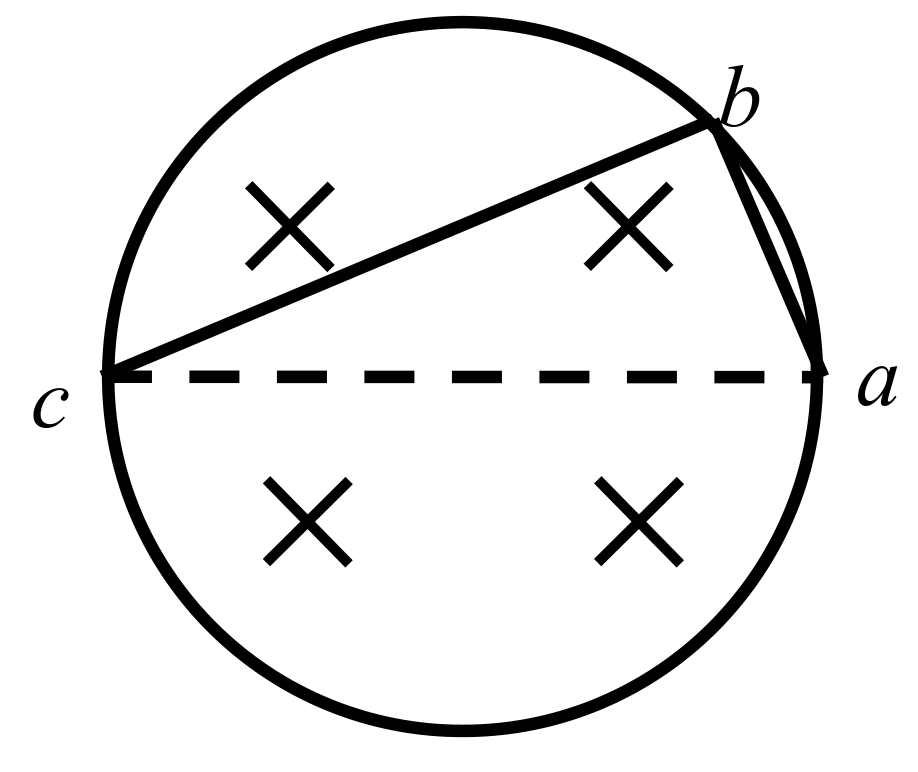
\includegraphics[width=5cm,height=4cm,keepaspectratio]{figures/magnet7.png}\par}\medskip

\end{document}
